\documentclass[twocolumn, 10pt]{article}
\usepackage{sectsty}
\usepackage{geometry}
\usepackage{amssymb}
\usepackage{yfonts}
\usepackage{graphicx,xcolor}

\newcommand*\sqding{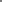
\includegraphics{square}}

\sectionfont{\fontsize{10}{12}\selectfont}


\geometry{
	a4paper,
	total={6.85in, 9.92in},
	left=0.71in,
	top=0.63in,
}
\usepackage[utf8]{inputenc}
\usepackage{hyperref}
\usepackage{listings}

\pagenumbering{gobble}

\title{\LARGE Trace memory references in your ELF PIE}
\author{Lorenzo Benelli}

\makeatletter
\newcommand{\fsize}{\f@size pt }
\newcommand{\textFontName}{\f@family}
\renewcommand{\maketitle}{
\begin{flushleft}
{\noindent\Huge\bf\@title}\break
\footnotesize\textit{poc-code: http://github.com/ltlollo/instr} \hspace*{\fill} \@author
\end{flushleft}
}
\makeatother


\begin{document}
\maketitle


Dear fellow cooks, have you ever wondered which positions of memory is your freshly baked x86 64 ELF
executable accessing? Here, follow this simple three-step recipe to find out how to check that, using
binary instrumentation!

\section*{\textfrak{I}ngredients (for one executable):}

\begin{itemize}
  \setlength\itemsep{0em}
  \item[$\sqding$] \textit{1} good disassembler (I suggest Capstone\textsuperscript{\tiny ®})
  \item[$\sqding$] \textit{1} good assembler (I suggest Keystone\textsuperscript{\tiny ®})
  \item[$\sqding$] \textit{5} memory pages at least, \textit{4}KiB (\textit{4.096}kB) each.
  \item[$\sqding$] \textit{1} function that dumps its input onto a file.
\end{itemize}

\section*{\textfrak{S}tep one: Find the code}

If the binary is not stripped, you can easily find its functions offsets and sizes, by looking inside
the elf's sections:
Locate the \textit{section header table} in your elf's header.
In the section headers find one with type \texttt{SHT\_SYMTAB} named \texttt{\textit{.symtab}} and
one with type \texttt{SHT\_STRTAB} named \texttt{\textit{.strtab}}.
In the \texttt{\textit{.symtab}}, the entries with type \texttt{STT\_FUNC}, are your functions, while
their names are in \texttt{\textit{.strtab}}.

\section*{\textfrak{S}tep two: Instrument}

Write a piece of position independent code that stores its input (\texttt{rax}) somewhere
(I'll call it \texttt{\textit{rax\_dump}}).
Personally, I like to place it after a page that I know I can write to, that, when full, I can dump
its content on disk.
Disassemble the code you found before and look for instructions of the form \texttt{op reg, [expr]},
\texttt{op reg, reg:[expr]}, \texttt{op [expr], reg}, or \texttt{op reg:[expr], reg}.
For each of them, generate a tiny gadget, using \texttt{lea rax, [expr]} to fetch the address, and
append it after the \texttt{\textit{rax\_dump}} you previously wrote.
Finally, replace the oringinal instruction with a jump to your new code, and you are all set.

\begin{figure}[h!]
\centering
\def\svgwidth{0.5\columnwidth}
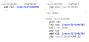
\includegraphics{ass}
\end{figure}

A couple of caveats: If your instruction is rip-relative remember to skip it or recompute its
destination, and offset your expressions by 8 if it uses \texttt{rsp}.

\begin{figure}
\centering
\def\svgwidth{0.5\columnwidth}

\includegraphics{gobbo}
\end{figure}

Also the instruction you are replacing might be smaller than a jump, so you may have to copy a bunch.
If you do so, remember to recompute the jumps internal to the original function.

\section*{\textfrak{S}tep three: Reassemble}

Adding our new stuff to the executable is not as easy as appending it, we also need to tell the
kernel where to map it into memory using program header entries.
So we are going to add a new copy of our original program header table with three new mappings: one
read only, with offset and address of the table itself (this so that the linker can also see it), one
R/W (so we can store some addresses), and one R/E pointing to the code we just generated. Beware of
mixing all these ingredients after the latest \texttt{vaddr+memsz} to avoid a confict with the
\textit{bss}, and that \texttt{vaddr-offset} must be 0 mod 4096, or just follow grandma's tip:
\textsl{keep all offsets and sizes in the program headers page-aligned}.

If you also wish to call some flushing code before the program shuts down, you'll need to append two
additional sections (and the respective R/W mappings as program headers entries).
A copy of \texttt{\textit{.fini\_array}} with the virtual address of your flushing code appended, and
a copy of \texttt{\textit{.rela.dyn}} with a new \texttt{R\_X86\_64\_RELATIVE} symbol pointing its
\texttt{r\_offset} and \texttt{r\_addend} to the file offset and address of your finalizer.
Don't forget to update all the \texttt{r\_offsets} of the other \texttt{R\_X86\_64\_RELATIVE} symbols
you moved with the \texttt{\textit{.fini\_array}} and update the \texttt{DT\_FINI\_ARRAY} and
\texttt{DT\_FINI\_ARRAYSZ} address and offset in the \texttt{\textit{.dynamic}} section.
Finally, update the \textit{program header table} offset in your elf's header
(and in the \texttt{PT\_PHDR} program header), with its new virtual address, et voilà, your binary
is ready to reveal its delicious secrets!

\textsc{\small Are you a professional chef? Then make sure to check out these professional tools for
instrumentation needs: \textbf{Pin}, \textbf{DynamicRIO}}

\end{document}
